\documentclass[12pt,a4paper]{article} % document setting, articles do not allow chapters
\usepackage[english]{babel} % english spell-check
\usepackage[utf8]{inputenc} % allows the input of special characters from keyboard
\usepackage[T1]{fontenc}
\usepackage{lmodern} %load modern fonts
\usepackage{helvet} % lead helvetica font
\renewcommand{\familydefault}{\sfdefault} % without this helvetica does not work on linux
\usepackage{textcomp} % for text symbols such as (C)
\usepackage{siunitx} % for mathematical embedding with $

\AtBeginDocument{\renewcommand{\bibname}{References}} % change Bibliography to Reference in TOC
\usepackage[compress]{natbib} % include bibliography
%super, numbers
\bibliographystyle{apalike} % simple bibliography style % sudo texhash
%\bibliographystyle{plainnat} %order by appearance: unsrtnat
\usepackage{hyperref} % allow printing URLs (here: for Bibliography)
\usepackage{cite}

\usepackage{graphicx} % include figures
\usepackage[labelfont=bf]{caption} % change figure caption to bold

\usepackage{titlesec} %change title style
\titleformat*{\section}{\normalsize\bfseries}
\titleformat*{\subsection}{\normalsize\itshape}

%\usepackage[mathlines]{lineno} % add line numbers
\usepackage{setspace} %for double spacing

\author{Masumi Stadler}
\title{PhD proposal}

%%%%%%%%%%%%
% Document %
%%%%%%%%%%%%
\begin{document}
%\linenumbers

\setlength{\parindent}{0cm}
Title (max 150 char): Diverging DNA and RNA communities along a boreal terrestrial-hydrological continuum (?) \\

Masumi Stadler\textsuperscript{1,*}, Paul A. del Giorgio\textsuperscript{1}\\

Affilitation:\\
(1) Groupe de Recherche Interuniversitaire en Limnologie (GRIL), Département des Sciences Biologiques, Université du Québec à Montréal, Montréal, QC, Canada


Institutional e-mail addresses: MS (stadler.masumi@courrier.uqam.ca), PdG (del\_giorgio.paul@uqam.ca)\\

Running title (max 50 char): Microbial communities along a boreal terrestrial-hydrological continuum.\\

*Contact corresponding author: Masumi Stadler \\
E-mail: m.stadler.jp.at@gmail.com \\
Phone: +1 (514)297-5330 \\
Address: Département des Sciences Biologiques, Université du Québec à Montréal, Case Postale 8888, Succursale Centre-Ville, Montréal, QC, H3C 3P8, Canada \\

Keywords: aquatic bacterial communities, terrestrial-aquatic continuum, ecosystem connectivity, residence time, boreal ecosystems, mass effects, environmental sorting, metacommunity, rare biosphere\\

Author contributions: PdG designed the sampling, MS collected the data, MS analysed the data, MS and PdG discussed the results and wrote the manuscript.\\

\newpage

\doublespacing

%\begin{abstract}


%\end{abstract}


\setlength{\parindent}{1cm}
\section*{Introduction}
(The Introduction should assume that the reader is knowledgeable in the field and should therefore be as brief as possible but can include a short historical review where desirable.)

Tralala

The consecutive flooding of the reservoirs creates a unique opportunity to study the transformation process of a running system into a standing water body. The shifts mainly imposed due to the increased residence times are likely to influence not only biogeochemical properties but also their microbial assemblages.

\section*{Material and methods}
\subsection*{Catchment characteristics and sampling design}
To follow the movement of microbial communities within a watershed, samples were taken along the Romaine river (C\^{o}te-Nord region, Qu\'{e}bec, Canada) (Fig. 1a-b) for three years from 2015-2017. The Romaine catchment belongs to the eastern black spruce-moss bioclimatic domain and drains an area (\textit{A}) of approximately 14 500 km\textsuperscript{2}. The catchment was glaciated 7 000 – 10 000 years ago and left mostly a till blanket and veneer as surficial material. It is mainly dominated by acid rocks (e.g. granodiorite, granite, quart diorite) with granitised sedimentary and volcanic rock, and has isolated patches of permafrost (0-10\%)(Natural Resources Canada). The soil is composed of roughly 61.4\% sand, 31.9\% silt, 6.7\% clay and stores approximately 140.4 t ha\textsuperscript{-1} of organic carbon (in top 5 cm; given are catchment averages)\citep{Lehner2013, Hengl2014}.

The river springs between the Atlantic and Saint Lawrence watersheds (52\textdegree{}52'20"N 63\textdegree{}36'55"W; 702 masl), and consequently flows through a series of lakes (hereafter headwater lakes) including the biggest lake in the catchment – Lake Br\^{u}l\'{e} (\textit{A}: 127.11 km\textsuperscript{2}, elevation: 470 masl). The river mainly flows towards the South with a maximum distance from the northern headwaters to the river mouth expanding to approximately 475.1 km. Nearly half of the catchment is covered by coniferous forests (\textit{P.mariana}-moss), with mixed forests being rather minor (11\%) and deciduous stands with white birch (\textit{Betula papyrifera}) and trembling aspen (\textit{Populus tremuloides}) are even more rare (2\%)\citep{HQreport2009}. The northern part of the catchment is characterised by a flat open black spruce (\textit{Picea mariana})-lichen forest with shrubs and moss-lichen (Fig. S1a). As one follows the river downstream, the relief changes drastically to a steep mountainous stretch that forms sections of canyons (Fig. S1b). The river looses 330 m of elevation from the mountainous section until it makes a sharp turn to the west into the lower coastal plain. The coastal plain is characterised by peatland areas with swamps and shallow waters that are completely permafrost free (Fig. S1c). There are two larger tributaries in the coastal plain that flow through the lakes Puyjalon (\textit{A}: 13.10 km\textsuperscript{2}) and Allard (\textit{A}: 19.24 km\textsuperscript{2}). A weather station located in the lower coastal plain (50\textdegree{} 16'55.000" N, 63\textdegree{} 36'41.000" W, Havre-Saint-Pierre Airport, Natural Resources Canada) recorded an annual precipitation of 810.77 $\pm$ 35.25 mm and 1.18 $\pm$ 0.73 \textdegree{}C, -32.63 $\pm$ 1.36 \textdegree{}C, and 25.8 $\pm$ 0.66 \textdegree{}C for mean, minimum and maximum temperature over the sampled years. 

The Romaine river has been dammed during the sampling period, forming a reservoir cascade complex with 4 reservoirs by 2020. The reservoirs Romaine 2 (RO2, \textit{A}: 81.15 km\textsuperscript{2}), Romaine 1 (RO1, \textit{A}: 13.22 km\textsuperscript{2}) and Romaine 3 (RO3, \textit{A}: 35.18 km\textsuperscript{2}) were flooded in the years 2014 (winter), 2015 (winter), and 2017 (spring), respectively.

Overall, 395 samples were collected for DNA (D) and 202 for RNA (R), covering spring (166-D, 69-R), summer (195-D, 99-R) and autumn (34-D, 34-R). RNA samples were sampled from 2016 onwards. To follow a terrestrial-aquatic continuum various sample types have been sampled (Table S1). Due to the remoteness and inaccessibility of the northern most headwaters, we have sampled the Petite Romaine sub-catchment (PR, \textit{A}: 310.73 km\textsuperscript{2}, elevation: 580 masl, Fig. 1c) that represents a headwater stream network. 

Surface soil samples were collected by mixing three randomly selected cores (30 cm) that were taken in proximity of installed piezometers to sample soil-water. The upper 5 cm including surface vegetation were removed before the soil was transferred into a sterile plastic bag. Three piezometers were randomly installed in proximity (30-100 cm) to a sampled stream with an average depth of 50 $\pm$ 20 cm. However, if the piezometers were installed too close to the stream main channel, hyporheic water was sampled instead. Piezometers were emptied 3 times (1-2 h) with a peristaltic pump before sample water was collected. The water from the randomly installed piezometers were pooled together. Groundwater was direcy collected from constructed wells with submersible pumps. Surface water samples were directly collected into a pre-rinsed carboy bottle at a depth of 0.5 m, close to the shore for stream samples and diverse locations within the river and reservoirs. Lake sediment samples were collected with sediment cores (1-2 m depth), and the upper 10 cm were collected and mixed for subsequent processing. All samples were stored at 4 \textdegree{}C upon arrival at the laboratory until further processing on the same day of sampling. 

\subsection*{Sample processing and sequencing}
Homogenised soil and sediment samples were transferred to aliquots of 0.25 g and frozen immediately on the same day of sampling. A minimum of 25 mL and 250 mL of soil-/hyporheic-water and surface water was filtered through 0.22 \si\micro m polycarbonate membrane filters (Merck Millipore, Darmstadt, Germany), respectively, and subsequently stored frozen. All DNA and RNA samples were frozen at -20 \textdegree{}C at the field station and further stored at -80 \textdegree{}C at the university laboratory until extraction. Samples for RNA extraction were submerged in RNAlater\textsuperscript{\textregistered} and LifeGuard\textsuperscript{\textregistered} Soil Preservation solution (QIAGEN\textsuperscript{\textregistered}, Hilden, Germany) for water and soil samples, respectively. To allow stabilisation, samples were left at 4 \textdegree{}C overnight and were subsequently stored frozen.

Following the manufacturers instructions, PowerWater\textsuperscript{\textregistered} and PowerSoil\textsuperscript{\textregistered} DNA and RNA extraction kits (MoBio, Carlsbad, CA, USA) were used to extract water and soil/soil-/hyporheic-water/sediment samples, respectively. In 2017, the equivalent DNeasy\textsuperscript{\textregistered} and RNeasy\textsuperscript{\textregistered} PowerWater\textsuperscript{\textregistered} Kits (QIAGEN\textsuperscript{\textregistered}) were used for DNA and RNA samples, respectively. cDNA was synthesised from the extracted RNA with a high capacity cDNA Reverse Transcription Kit (Applied Biosystems\textsuperscript{\texttrademark}, Foster City, CA, USA). Successful extraction was evaluated via PCR amplification of the 515F-806R primers (IDT Technologies, Coralville, IA, USA) and DNA concentration was measured with a NanoDrop 2000c (Thermo Fisher Scientific Inc., Waltham, MA, USA). Extracts were sent to G\'{e}nome Qu\'{e}bec Innovation Centre (Montr\'{e}al, QC, Canada) for paired-end metabarcoding of the 16S rRNA V4 region using the primers 515F (5'-GTGCCAGCMGCCGCGGTAA-3') and 806R (5'-GGACTACHVGGGTWTCTAAT-3') on a Illumina MiSeq (PE250) platform.

\subsection*{Bioinformatic analysis}
Primers were removed using the software \textit{cutadapt} (Version 1.18, \citet{Martin2013}), which allows for the removal of the primer sequence and its variants in their true and complement orientations. Additionally, all reads shorter than 125 nucleotides were removed as they cannot achieve a minimum overlap necessary for paired-end merging in downstream processing.

To identify amplicon sequence variants (ASVs), 16S rRNA amplicon reads were analysed through the DADA2 (Divisive Amplicon Denoising Algorithm 2) pipeline (Version 1.14.1, \citet{Callahan2017}) on R Version 3.6.3 \citep{RCoreTeam2017}). Read qualities were evaluated for each sequencing plate separately and read length was trimmed according to their quality scores. The most conservative trimming criteria still allowed for an overlap of forward and reverse reads by 60 bp. Samples were pooled by plate, season and sequencing depth for learning the error rates. DADA2 runs on a sample by sample basis, and thus removes observed singletons by sample to avoid inclusion of false-positive sequencing errors. To retain more rare taxa within a sampling campaign (year-season combinations) along the continuum, samples were 'pseudo'-pooled for the \textit{dada()} step.  This step enables the removal of singletons by pool but retains singletons within a sample. Paired-ends were merged after successful inference of amplicon variants. Subsequently, chimeras were removed (\textit{removeBimeraDenovo()}) and all ASVs that are identical in sequence but differ only by length were merged together with \textit{collapseNoMismatch()}, leading to ASVs that represent a unit similar to 100\% similar operational taxonomix units. Finally, taxonomy was assigned with the \textit{DECIPHER} package (Version 2.14.0, \citet{Wright2016}) implementing the increased accuracy IDTAXA algorithm \citep{Murali2018} and the provided trained classifier of the SILVA database (Version 138, \citet{Pruesse2007}).

All ASV observations with less than 10 reads per sample were removed. Furthermore, \textit{metagenomeSeq} was used to transform and stabilise variation in library sizes with cumulative sum scaling (CSS) \citep{Paulson2013}. For alpha diversity estimations, CSS results were rounded to its integer to represent count data necessary for alpha-diversity calculations. CSS results were compared with results achieved with various rarefaction thresholds. To account for random sampling effects, rarefaction was conducted with 100 random iterations. Similarly to the CSS data treatments, the mean of all iterations was rounded to its integer to be used for subsequent analysis. There were no substantial differences in the results between CSS and various rarefaction thresholds (Fig. S2). Consequently, CSS results were used for downstream analyses for consistency.

\subsection*{Data handling and statistical analyses}

The packages \textit{phyloseq}, \textit{tidyverse}, \textit{plyr} and \textit{data.table} were used for data wrangling and transformation \citep{McMurdie2013,Wickham2019, Wickham2011, Dowle2019}, and \textit{doMC} enabled parallel processing \citep{Analytics2019}. Distance and diversity metrics were calculated using \textit{vegan}, and \textit{ape} was used to compute the PCoA \citep{Oksanen2017, Paradis2018}. \textit{ggplot2}, \textit{ggpubr} and \textit{ggnewscale} were used to visualise the results \citep{Wickham2016, Kassambara2018, Campitelli2020}. All analyses have been conducted in R \citep{RCoreTeam2017} and RStudio \citep{RStudioTeam2016}. Maps were created with QGIS (version 3.12) and a digital elevation model (Natural Resources Canada). Watersheds were delineated with ArcMap (version 10.5.1) and the Spatial Analyst Toolbox. 

\section*{Results}

\section*{Discussion}

\subsection*{Data accessibility}
DNA and RNA sequences have been archived (database name and number). The code and meta data to produce this manuscript are available at \url{https://github.com/masumistadler/catchment_microbial_community}. \\

\section*{Conflict of Interest}
The authors declare no conflict of interest.

\section*{Acknowledgements}
We are especially grateful to Alice H. Parkes, Annick St-Pierre, and Serge Paquet, who maintained and oversaw the project over the years. Collection and analysis of all variables would have not been possible without the support from members of the CarBBAS team including great contributions from undergraduate students. Therefore, we would like to thank Felipe Rust, Clara Ruiz-Gonz\`{a}lez, Trista Vick-Majors, Alexandre Ducharme, Roy Nahas, Ryan Hutchins, Marie Laure G\'{e}rardin,  Erin Hotchkiss, Karelle Desrosiers, Martin Demers, Sara Mercier Blais, Julia Jakobsson, Francesca del Giorgio, Brenden Chabot, Sebastian Dugas, and Pascale Ouimet. We would also like to thank Katherine Velghe and Marilyne Robidoux for laboratory assistance and Mario Muscarella for insightful discussions on the results. We also thank xx anonymous reviewers for constructive comments that improved the manuscript. This study is part of the program of the Carbon Biogeochemistry in Boreal Aquatic Systems (CarBBAS) Industrial Research Chair, co-funded by the Natural Science and Engineering Research Council of Canada (NSERC) and Hydro-Qu\'{e}bec.

\newpage
\singlespacing

\bibliography{/media/shared/Documents/University/PhD/BibTEX/LR_miccom_paper}

\newpage
\section*{Figure legends}
Figure 1. \textbf{Location and overview of the La Romaine catchment}. a) Scale and overview of the whole La Romaine catchment. Samples are represented as points. b) Location of the catchment within Canada and Québec. c) Focus on all built reservoirs RO1 (2015), RO2 (2014) and RO3 (2017) and the headwater stream sub-catchment Petite Romaine (PR).

\section*{Tables}

\section*{Figures}
\begin{figure}[!ht]
\centering
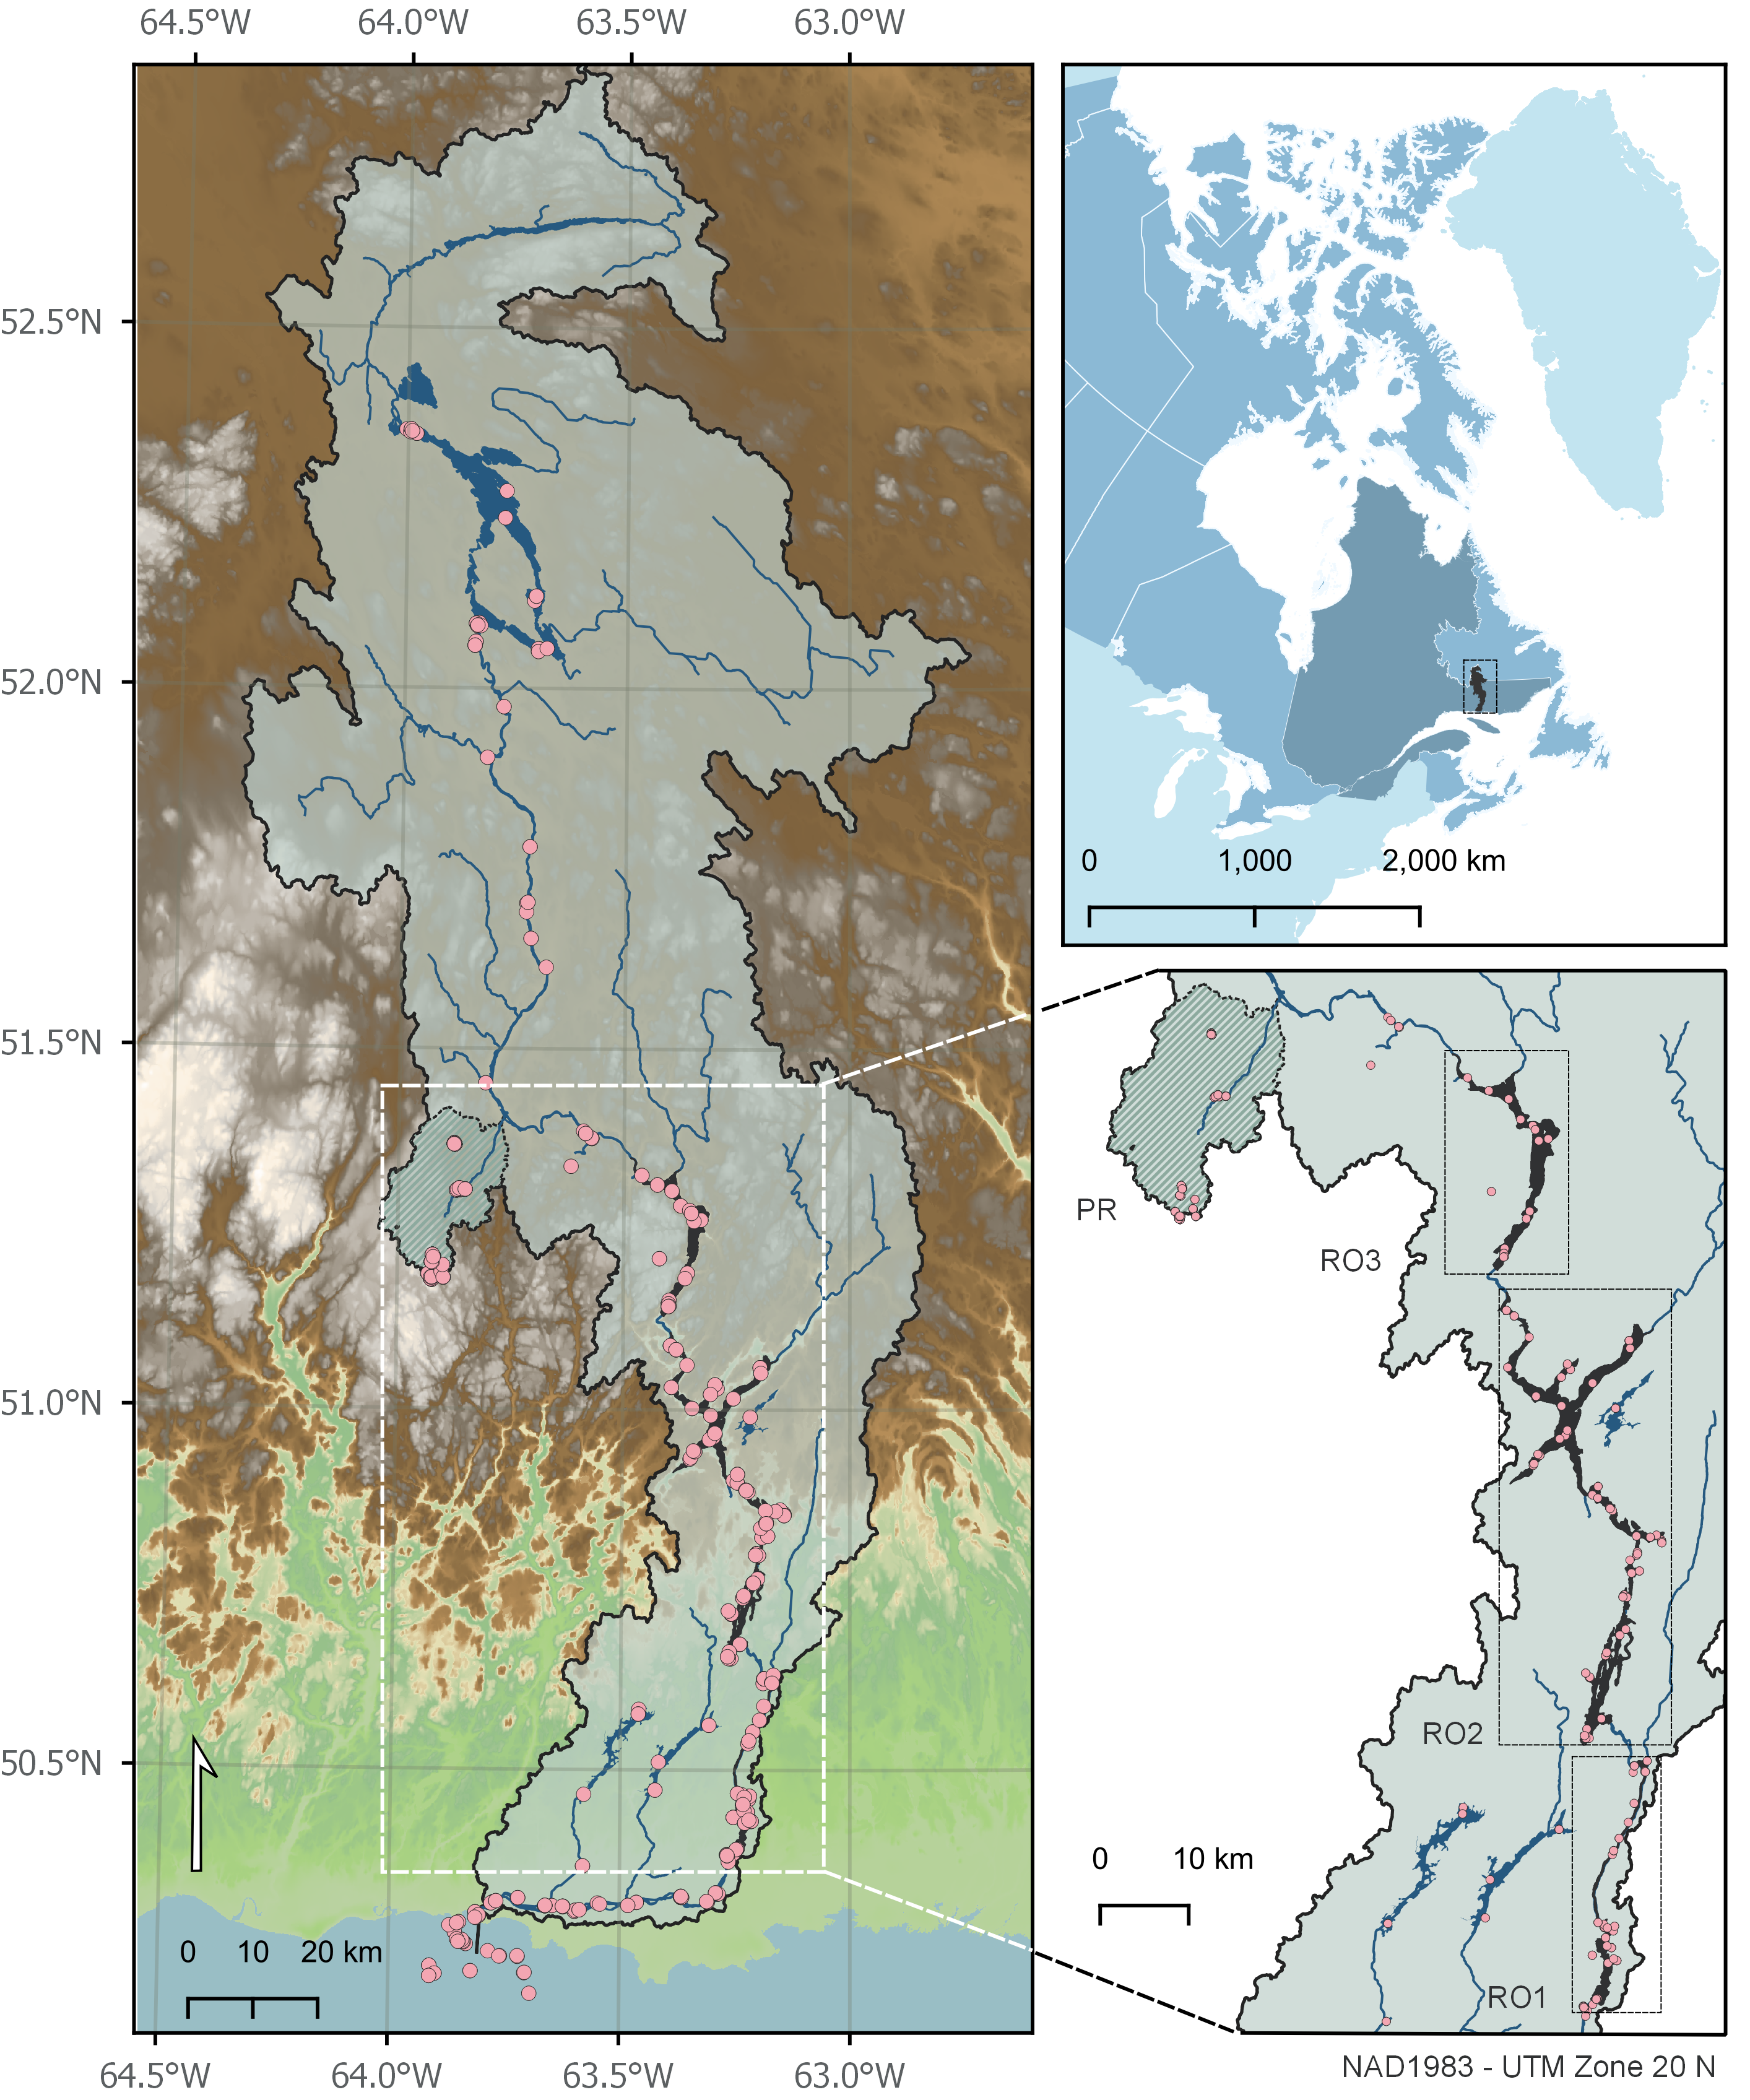
\includegraphics[width=12cm]{../Figures/LR_miccom_paper_threemaps.png}
\caption{\textbf{Location and overview of the La Romaine catchment}. a) Scale and overview of the whole La Romaine catchment. Samples are represented as points. b) Location of the catchment within Canada and Québec. c) Focus on all built reservoirs RO1 (2015), RO2 (2014) and RO3 (2017) and the headwater stream sub-catchment Petite Romaine (PR).}
%includegraphics[width=1\textwidth]
\end{figure}

\end{document}
